% questions.tex —— 1977 年·安徽卷（理科） · 题目内容片段（无答案）
% 由 tools/generate_projects.py 依来源总账自 1977/1977_数学真题_安徽理_试题.md 生成，勿手改（改源 MD 后重跑）


\gkpart{高等学校招生（理工科）数学试题}

\begin{gktip}
\textbf{来源说明}：本题面依据固定源 PDF《1977 安徽理》第 1—3 页逐题转录，原卷页首标题为「安徽省 高等学校招生（理工科）数学试题」，页底印刷页码依次为「数学—52」「53—数学」「数学—54」。源卷为题面与解答合订的扫描材料：第 4 页为附加题手绘插图（旁注「安，加．」），第 5—13 页为「安徽省 高校考试（理科）数学试题 解答及评分标准（原试题均略）」（印刷页码 题解—20 至 题解—28），故配套答案与解析由本库对照该解答独立复算与推导，\textbf{非官方标准答案}。正式题共 8 道，其中第八题两小题选作一题，原卷小题印作「1.」「2.」，本库按小问连续编号规范重排为（1）（2）；末尾〔附加题〕原卷未编号，本库顺延编为附加题 9，不计入正式题量。各题分值按原卷照录：第一题题首标注「本题满分 20 分，每小题 3 分」，按 7 个小题每小题 3 分应为 21 分，与满分 20 分不一致，系源卷自身矛盾，见第一题源注。
\end{gktip}

\begin{question}
\gkti{1}\textbf{（本题满分 20 分，每小题 3 分）} 

\begin{gktip}
\textbf{源注}：原卷题首即标注「本题满分20分，每小题3分」；7 个小题按每小题 3 分计应为 21 分，与满分 20 分不一致，源卷两数并存，本文照录。
\end{gktip}

\Needspace{5\baselineskip}
（1） 计算：

\nopagebreak[4]
\[
0.25\times(-2)^2-4\div(\sqrt5-1)^0-\left(\frac16\right)^{-\frac12}+
\]

\nopagebreak[4]
\[
+\frac{\sqrt3}{\sqrt3-\sqrt2};
\]

\begin{gktip}
\textbf{源注}：原卷此式跨行排印，行末与行首各印一个加号；按数学含义应只有一个加号，本文两处照录，计算按一个加号处理（源解答亦如此）。
\end{gktip}

（2） 求函数 $y=\log_a(4^x-16)$ 的定义域；

（3） 求 $\sin(-915^\circ)$ 的值；

（4） 求函数 $y=\arcsin(1-2x)$ 的定义域；

（5） 化复数 $-1+i$ 为三角函数式；

（6） 化简 $\sin A\cdot\sqrt{1-\sin^2A}$ （$90^\circ<A\leqslant180^\circ$）

\begin{gktip}
\textbf{源注}：原卷题面印作「sinA·√(1$-$sin²A)」，源卷解答部分却按「secA·√(1$-$sin²A)」展开并得 $-$1，两处不一致；本文按题面照录，解析中按题面化简并附源解答口径的结果。
\end{gktip}

（7） 已知元锥的母线长 3 cm，底面直径 2 cm，求它的侧面积（$\pi$ 取 3.14）。

\begin{gktip}
\textbf{源注}：「元锥」为原卷用字（源解答部分作「园锥」），即圆锥，本文照录。
\end{gktip}

\Needspace{0.4\textheight}
\end{question}
\begin{question}
\gkti{2}\textbf{（本题 9 分）} 

用宽为 80 厘米的铁皮制作一个槽，槽的截面 $ABCD$ 是一个矩形。

（1） 求槽的截面积 $y$ 关于槽深 $x$ 的函数关系式；

（2） 求出这个函数圆象的顶点坐标、对称轴方程；

\begin{gktip}
\textbf{源注}：原卷印作「函数圆象」，应为「图象」之误排，本文照录。
\end{gktip}

（3） 当槽深为多少厘米时，槽的截面积最大？这个最大面积是多少平方厘米？

\begin{gktip}
原源 PDF 第 2 页题首附有槽的立体示意图（旁注「安，二」）；LaTeX 版按源图重绘。
\end{gktip}
\nopagebreak[4]
\begin{center}% 1977 年安徽卷（理科）第 2 题：铁皮槽立体示意图，截面矩形 ABCD（A 左上、B 左下、C 右下、D 右上），
% 槽口两斜棱在远端交汇，其间按原卷标注 π/6 角（按源卷第 2 页「安，二」图布局重绘）
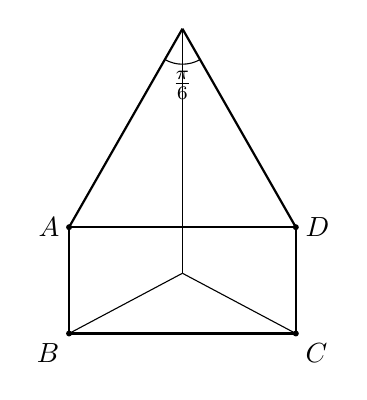
\begin{tikzpicture}[scale=0.9]
  % 前面板矩形
  \coordinate (A) at (0,1.5);
  \coordinate (B) at (0,0);
  \coordinate (C) at (3.2,0);
  \coordinate (D) at (3.2,1.5);
  % 远端顶点（手绘原图将远端上下棱各收缩为一点）
  \coordinate (P) at (1.6,4.3);
  \coordinate (Q) at (1.6,0.85);
  \draw[thick] (A)--(B)--(C)--(D);
  \draw[thick] (A)--(P);
  \draw[thick] (D)--(P);
  \draw[thin]  (B)--(Q);
  \draw[thin]  (C)--(Q);
  \draw[thin]  (P)--(Q);
  \draw[thick] (A)--(D);
  \fill (A) circle (1.2pt) node[left] {$A$};
  \fill (B) circle (1.2pt) node[below left] {$B$};
  \fill (C) circle (1.2pt) node[below right] {$C$};
  \fill (D) circle (1.2pt) node[right] {$D$};
  % 槽口两斜棱夹角标注（原卷标注 π/6，题面与解答未使用，按原样保留）
  \draw (P) ++(240.3:0.5) arc[start angle=240.3, end angle=299.7, radius=0.5];
  \node at (1.6,3.5) {$\frac{\pi}{6}$};
\end{tikzpicture}
\end{center}
\nopagebreak[4]
\end{question}
\begin{question}
\gkti{3}\textbf{（本题 12 分，每小题 6 分）} 

（1） 写出 $\left(\sqrt[3]{x}-\dfrac{2}{3\sqrt[5]{x}}\right)^n$ 的展开式中的第 $(r+1)$ 顶；

\begin{gktip}
\textbf{源注}：原卷印作「第 $(r+1)$ 顶」，「顶」应为「项」之误排，本文照录。
\end{gktip}

\Needspace{5\baselineskip}
（2） 设 $AM$ 是直角三角形斜边 $BC$ 上的中线，求证：

\nopagebreak[4]
\[
BC^2+AC^2+AB^2=8AM^2.
\]

\end{question}
\begin{question}
\gkti{4}\textbf{（本题 18 分，1.题 8 分，2.题 10 分）} 

\Needspace{5\baselineskip}
（1） 化简

\nopagebreak[4]
\[
\sqrt{5^{2\log_5(\lg x)}-2\lg x+1};
\]

\Needspace{5\baselineskip}
（2） 求下面数列的前 $n$ 项的和：

\nopagebreak[4]
\[
\lg\frac13+\lg\frac{10}{3^2}+\lg\frac{100}{3^4}+\lg\frac{1000}{3^8}+\cdots\cdots.
\]

\end{question}
\begin{question}
\gkti{5}\textbf{（本题 10 分）} 

已知 $\triangle ABC$ 的三个内角 $A\text{、}B\text{、}C$ 成等差数列，且最大角与最小角的对边之比是 $(\sqrt3+1):2$，试求此三角形三个内角的度数。

\end{question}
\begin{question}
\gkti{6}\textbf{（本题 10 分）} 

设 $P(8,2)$ 为平面直角坐标系上一点，$y^2=x$ 是曲线，$y-x-1=0$ 是一直线。

（1） 求过 $P$ 点与直线 $y-x-1=0$ 平行的直线方程；

（2） 求所求的直线已知曲线交点的坐标；

\begin{gktip}
\textbf{源注}：原卷印作「求所求的直线已知曲线交点的坐标」，「直线」后疑脱「与」字（应为「与已知曲线交点」），本文照录。
\end{gktip}

（3） 作出它们的图象。

\end{question}
\begin{question}
\gkti{7}\textbf{（本题 10 分）} 

判断下列方程的轨迹，并画出象：

\begin{gktip}
\textbf{源注}：原卷印作「并画出象」，疑脱「图」字（应为「画出图象」），本文照录。
\end{gktip}

\nopagebreak[4]
\[
25x^2-14xy+25y^2-288=0.
\]

\Needspace{0.4\textheight}
\end{question}
\begin{question}
\gkti{8}\textbf{（本题两小题选作一题，满分 10 分）} 

（1） 用 0 到 9 这十个数字可以排成多少个含有两个重复字的三位数？

（2） 利用数学归纳法证明 $x^n-y^n$ 能被 $x-y$ 整除（$n$ 为自然数）。

\begin{gktip}
\textbf{题号说明}：原卷第 8 题两小题印作「1.」「2.」（两小题选作一题）。本库题库规范要求小问连续编号，故重排为（1）（2），未增删题干内容。
\end{gktip}

\textbf{附加题 9．（满分 20 分）}

\begin{gktip}
\textbf{题号说明}：原卷此题栏名「〔附加题〕」，未编号；本库按正式题后顺延编号为附加题 9，不计入正式题量。
\end{gktip}

\Needspace{5\baselineskip}
如图，在矩形 $ABCD$ 中，$A_1E\parallel AB$，$AA_1=A_1A_2=A_2A_3=A_3A_4=A_4D=a$，$AB_1=B_1B_2=B_2B=\sqrt3\,a$。试用三种方法证明：

\nopagebreak[4]
\[
\angle B_1A_1E+\angle B_2A_1E+\angle BDC=\frac{\pi}{2}
\]

（注：三种方法是指每种方法各以代数、三角、几何知识为主来证明）

\begin{gktip}
原源 PDF 第 4 页附有矩形分割手绘插图（旁注「安，加．」）；LaTeX 版按源图重绘。
\end{gktip}
\nopagebreak[4]
\begin{center}% 1977 年安徽卷（理科）第 9 题（附加题）：矩形 ABCD 分割示意图，
% AD 边上 A1—A4 五等分（AA1=…=A4D=a），AB 边上 B1、B2 三等分（AB1=B1B2=B2B=√3a），
% 过 A1 作 AB 的平行线交 BC 于 G，E 在该线上 B1 的正上方（B1E⊥AB），
% 连线 A1B1、A1B2（按源卷第 4 页「安，加．」手绘图布局重绘）
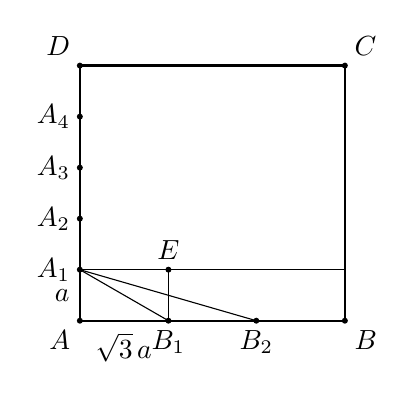
\begin{tikzpicture}[scale=0.9]
  \coordinate (A) at (0,0);
  \coordinate (B) at (3.74,0);
  \coordinate (C) at (3.74,3.6);
  \coordinate (D) at (0,3.6);
  \coordinate (A1) at (0,0.72);
  \coordinate (A2) at (0,1.44);
  \coordinate (A3) at (0,2.16);
  \coordinate (A4) at (0,2.88);
  \coordinate (B1) at (1.25,0);
  \coordinate (B2) at (2.49,0);
  \coordinate (E) at (1.25,0.72);
  \coordinate (G) at (3.74,0.72);
  \draw[thick] (A)--(B)--(C)--(D)--cycle;
  \draw[thin] (A1)--(G);
  \draw[thin] (A1)--(B1);
  \draw[thin] (A1)--(B2);
  \draw[thin] (B1)--(E);
  \fill (A) circle (1.2pt) node[below left] {$A$};
  \fill (B) circle (1.2pt) node[below right] {$B$};
  \fill (C) circle (1.2pt) node[above right] {$C$};
  \fill (D) circle (1.2pt) node[above left] {$D$};
  \fill (A1) circle (1.2pt) node[left] {$A_1$};
  \fill (A2) circle (1.2pt) node[left] {$A_2$};
  \fill (A3) circle (1.2pt) node[left] {$A_3$};
  \fill (A4) circle (1.2pt) node[left] {$A_4$};
  \fill (B1) circle (1.2pt) node[below] {$B_1$};
  \fill (B2) circle (1.2pt) node[below] {$B_2$};
  \fill (E) circle (1.2pt) node[above] {$E$};
  \node at (0.62,-0.38) {$\sqrt3\,a$};
  \node at (-0.25,0.36) {$a$};
\end{tikzpicture}
\end{center}
\nopagebreak[4]

\end{question}